\chapter{User interface design}
\label{chap:user_interface_design}
When designing a user interface with the intention of reaching a high level of usability, a systematic approach is key. The process we have used, can be roughly divided in to 4 steps, where the latter part can be repeated until the Quality Requirements, listed in \ref{subsec:quality_requirements}, have been met. \cite{lauesen} \\
The steps are:
\begin{enumerate}
\item Analysis of users and tasks
\item Construct prototype
\item Perform usability tests
\item Amend prototype 
\end{enumerate}

This chapter have been split into two parts due to the differences between them. We will provide a detailed walkthrough of the process for an element in each part, and the full history of mockups can be found in \ref{app:mockups}.
\section{Prototypinng}
\label{sec:prototyping}
\todo{relevance? rename/move/divide}
When designing a prototype, there is no systematic way of deciding how many screens are needed, and what they need to contain \cite{lauesen}.


What does exist, is conventions and typical behaviour, so we have tried to utilize this to construct a wireframe design for the frontpage \cite{garrett}. The wireframe seen on figure \ref{fig:wireframe_frontpage} is what later evolved to our main view.

Based on the user and task analysis conducted in \ref{chap:analysis}

\begin{figure}[htb]
\begin{center}
\leavevmode
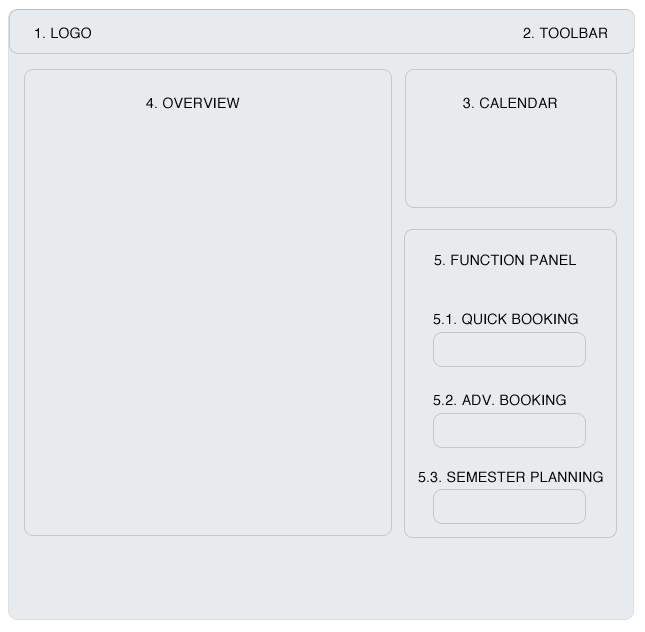
\includegraphics[width=0.6\textwidth]{images/wireframe1}
\end{center}
\caption{Wireframe for the frontpage}
\label{fig:wireframe_frontpage}
\end{figure}

\begin{itemize}
	\item \textbf{1. Logo}\\
	The logo for the application, which by convention should be located in the top left corner and link to the frontpage. \cite{steve}
	\item \textbf{2. Toolbar}\\
	A navigation toolbar. Should be used to login and logout, and for accessing the personal user account overview.
	\item \textbf{3. Calendar}\\
	An object used to navigate to a specific day in the future (or past).
	\item \textbf{4. Overview}\\
	The main overview, which should present a map of the university.
	\item \textbf{5. Function panel}\\
	A panel containing buttons used to enter the booking interface, or the semester planning.
\end{itemize}

\section{Usability tests} % (fold)
\label{sec:usability_tests}
%%%% MENTION SOMETHING ABOUT SCENARIOS %%%%

% section usability_tests (end)


\section{Design process}
\label{sec:design_process}

\subsection{Design of the day to day booking interface}
For a full history of our mockups, please refer to %\ref{app:mockups}

\begin{figure}[htb]
\begin{center}
\leavevmode
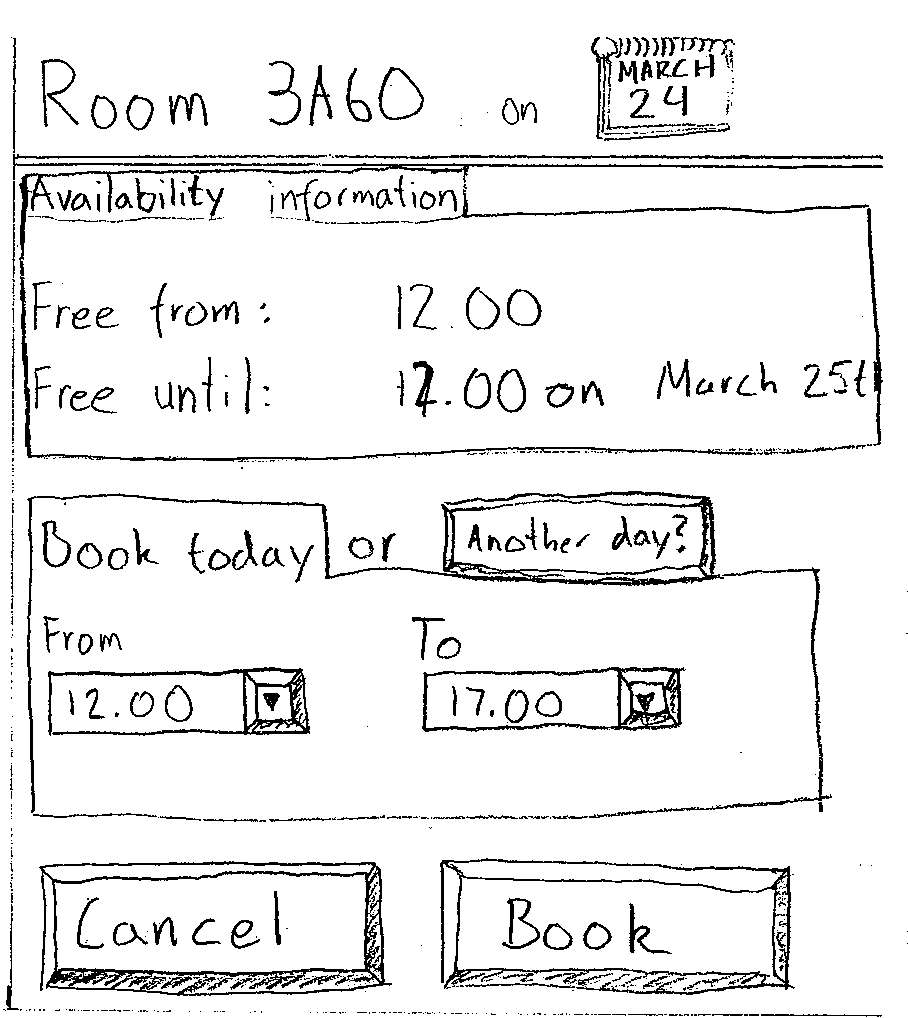
\includegraphics[width=0.6\textwidth]{images/bookRoomMockup}
\end{center}
\caption{First draft of the simple booking panel}
\label{fig:book_room_mockup}
\end{figure}

Seen on figure \ref{fig:book_room_mockup} is the lower right panel of the main screen, which was thought to be in charge of all interaction, trying to give the user the impression that they never left the homepage, and to make sure no-one got lost in subscreens and menus. Our first usability tests quickly revealed that we had been mistaken. All the test subjects felt overwhelmed by the amount of options, and due to all the clutter did not spot the vital functions.

\begin{figure}[htb]
\begin{center}
\leavevmode
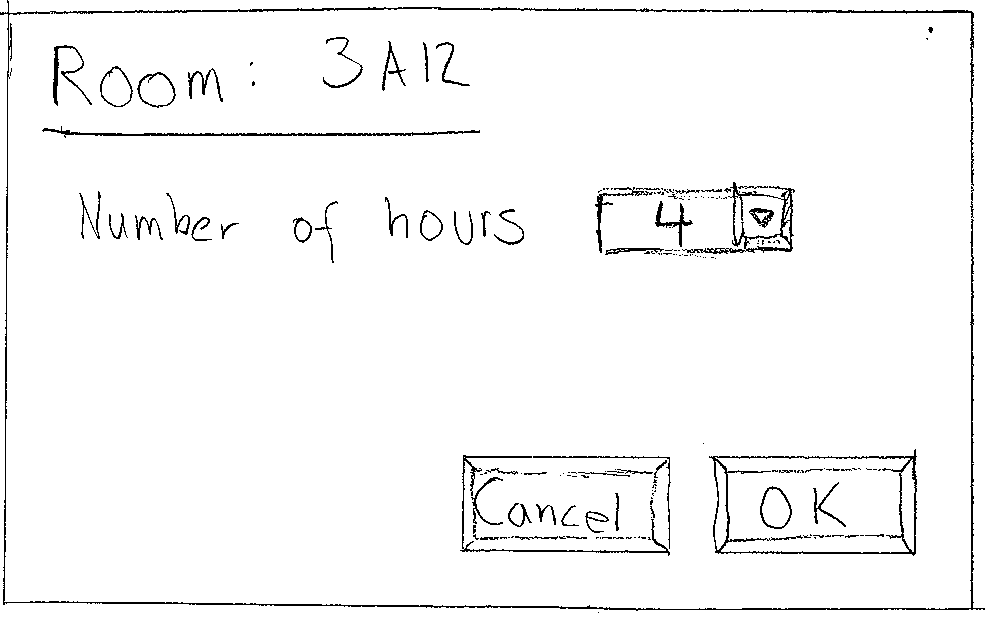
\includegraphics[width=0.8\textwidth]{images/bookRoomMockup2}
\end{center}
\caption{Second attempt at the simple booking. This time as a window overlaying the main view.}
\label{fig:book_room_mockup2}
\end{figure}

Second time around, we tried making it as basic as possible and simply presenting the user with a dialog (not a pop-up, just an overlay) for selecting how many hours from now the room should be booked. The flaw with this was that noone was able to figure out the availability of a room in the near future. This is when we realized that the best successes we've had with room booking was the first draft of the week-overview screen.

\begin{figure}[htb]
\begin{center}
\leavevmode
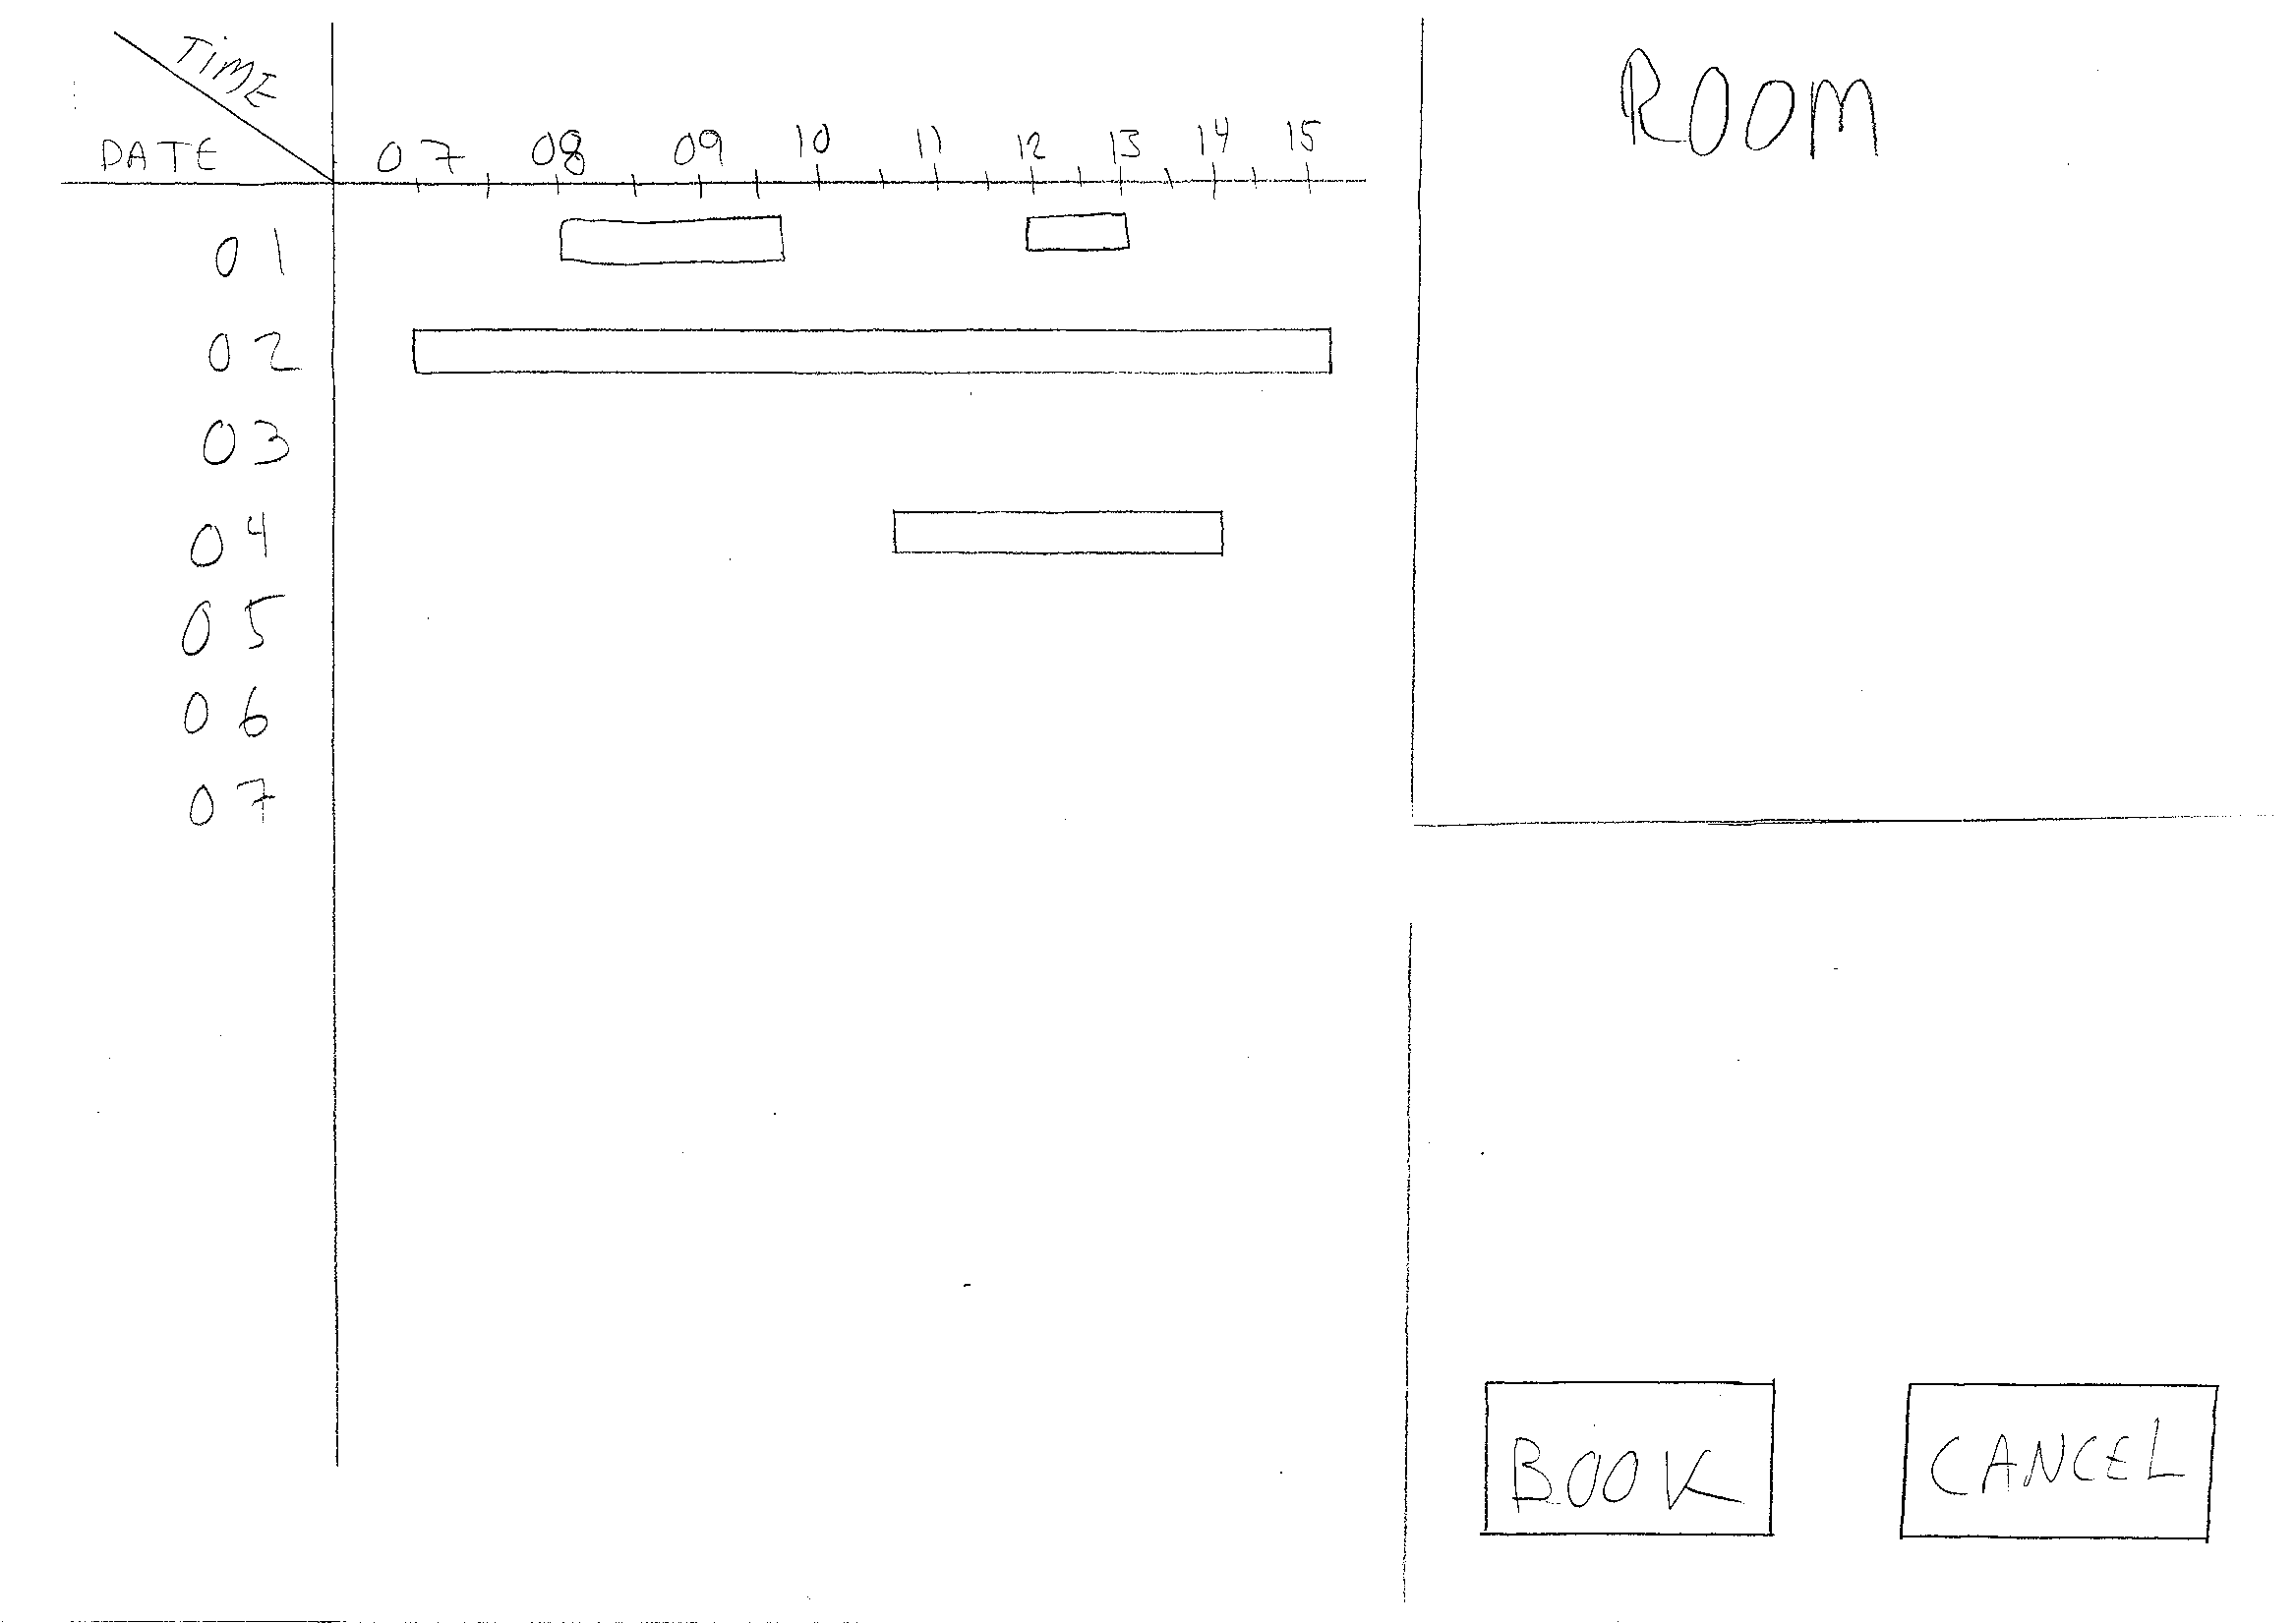
\includegraphics[width=0.8\textwidth]{images/weekMockup}
\end{center}
\caption{The mockup screen for a week overview on a specific room.}
\label{fig:week_mockup}
\end{figure}

All the test subjects used the 'matrix' overview shown on figure \ref{fig:week_mockup} both creatively and effectively, so we decided to try and utilize that success to the maximum by redirecting even a simple booking task to the same screen.
The only exception we have made to this is when using the "book now"-functionality, which will simply book a room for 4 hours and notify the user which one they have been assigned, with the ability to either accept or reject.

\begin{figure}[htb]
\begin{center}
\leavevmode
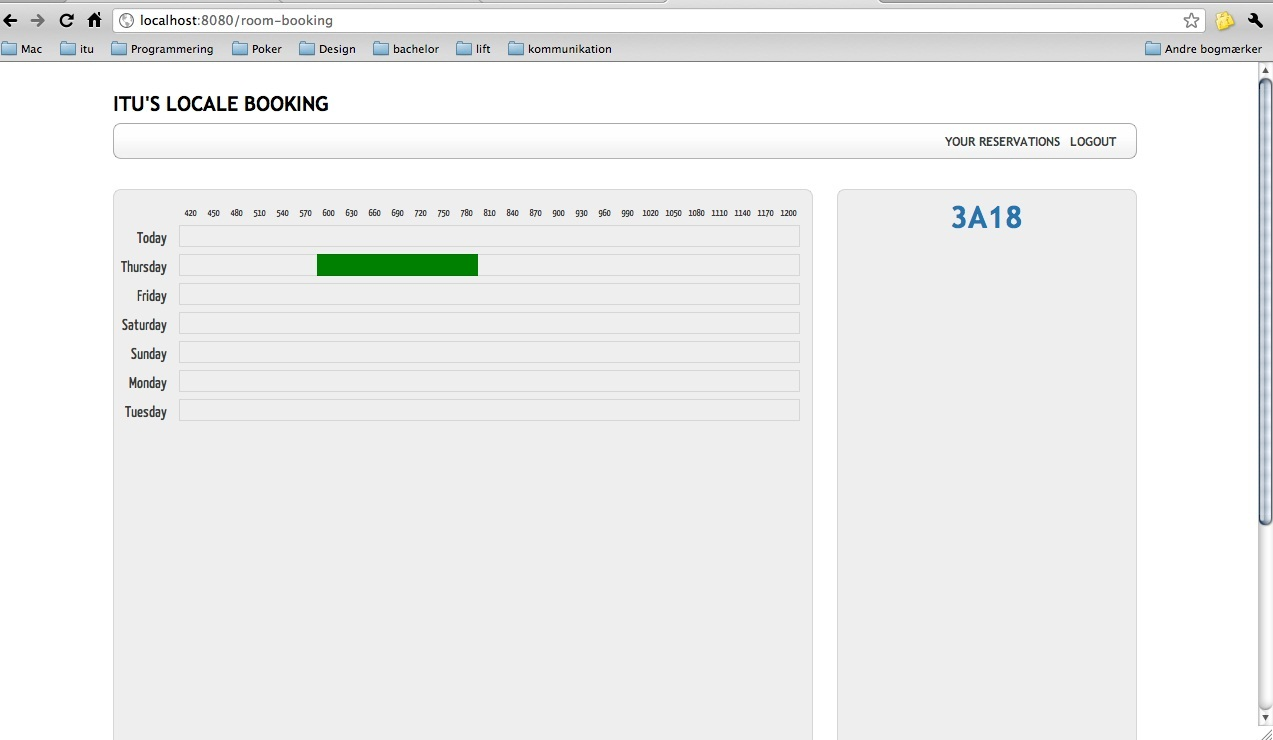
\includegraphics[width=1\textwidth]{images/weekFinal}
\end{center}
\caption{The almost finished screen for a week overview on a specific room.}
\label{fig:week_final}
\end{figure}

The final design to book a room, as shown on figure \ref{fig:week_final}, grants an availability overview of 7 days, starting with the current day. Through our tests, we noted test subjects trying to drag the mouse to select, and others clicking for a start time followed by a click on end time, so we have chosen to allow for both.
To assist the user in figuring out how it works, we have added highlighting of both the day and time when mouse is moved across the matrix.

Søren Lauesens first law of usability\cite{lauesen} states that a heuristic evaluation of usability flaws only has a 50\% hit-rate, which we admittedly found out was the case. We anticipated that our first design might be too dense, but never guessed that the wider overview proved more efficient for a simple booking.
\todo{fix it}


\subsection{Layout}
%maybe move?
Being a website poses some extra considerations - namely those of browsing habits. Two examples we will refer to, and assume basic familiarity with, in this section are wikipedia.org and google.com
%kan dette bruges?
\todo{ indsæt små billeder af wikipedia og google med F-pattern eyetrack }

%Let us for a second imagine a search for 'random' was made on both those pages. According to research by Jakob Nielsen (---- indsæt ref), users tend to scan the page in a pattern slightly resembling a capital F, ignoring banners and everything that looks like 'off-site' content.

\section{Proposed design}
\label{sec:proposed_design}
\todo{Explain and illustrate the proposed design}
